%!TEX root = ../thesis.tex
%*******************************************************************************
%****************************** Third Chapter **********************************
%*******************************************************************************

\chapter{Data Description}%
In this chapter, we will see an overview of the starting data used in this research, as well as some general statistics about it.

\section{Where the data comes from}
The data are tweets collected from the Twitter API containing the hashtag \#cop21 \#cop26. 
For each cop, we have two jsonlines files, one for the tweets and one for the users involved. The fields are the ones stated in the documentation \footnote{ \href{https://developer.twitter.com/en/docs/twitter-api/data-dictionary/object-model/tweet}{https://developer.twitter.com/en/docs/twitter-api/data-dictionary/object-model/tweet}}, there are many but the relevant ones to us are the following: 

\begin{table}[H]
\centering
\begin{tabular}{|l|l|}
\hline
\textbf{Field} & \textbf{Description} \\ \hline
author & The ID of the author \\ \hline
author\_name & The username of the author \\ \hline
text & The text of the tweet \\ \hline
date & The creation date of the tweet \\ \hline
lang & The language of the tweet \\ \hline
conversation\_id & The ID of the conversation the tweet belongs to \\ \hline
referenced\_type & The type of the referenced tweet \\ \hline
referenced\_id & The ID of the referenced tweet \\ \hline
mentions\_name & The usernames of the mentioned users in the tweet \\ \hline
mentions\_id & The IDs of the mentioned users in the tweet \\ \hline

\end{tabular}
\caption{Description of the fields used of the tweets data}
\label{tab:my_label}
\end{table}
While we use the user's file to map the ID of the users to their username, even though we do not always have this information, in that case, we use the user ID as the username.

\section{Some statistics}
We have data from 2 cops: COP21, COP26.
All the tweets are in English and without links or image/video content.
We call an original tweet a tweet written by a user, so that's not a retweet. Fig \ref{fig:tweets_by_date} shows the distribution of the tweets over time for both cops; most of the tweets have been tweeted while the conferences were taking place.

\begin{figure}[H]
    \centering
    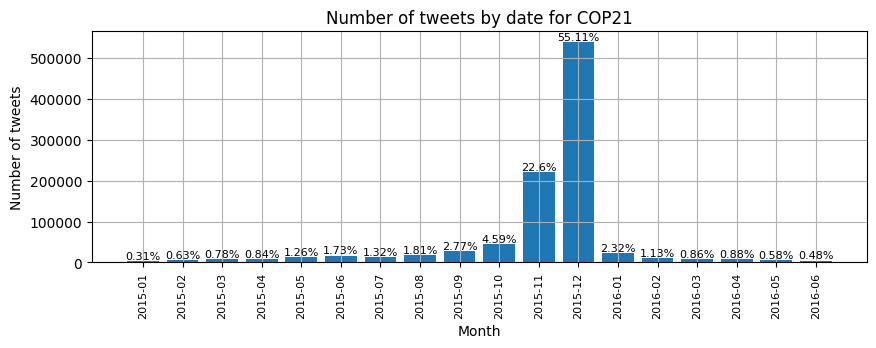
\includegraphics[width=0.75\linewidth ]{Chapter3/figures/tweets_by_date_cop21.png}

    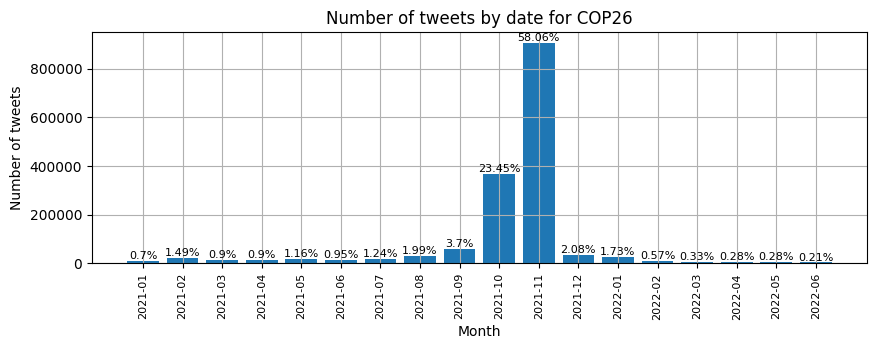
\includegraphics[width=0.75\linewidth ]{Chapter3/figures/tweets_by_date_cop26.png}
    \caption{Numebr of tweets by date for cop 21 and cop26}
    \label{fig:tweets_by_date}
\end{figure}

\paragraph{COP21}
The tweets span from January 2015 to June 2016, but 77\%  of the tweets are from November and December 2021; cop26 was held between 30th November and 12th December. In the dataset, 975040 tweets have been tweeted by 234389 users, of which only {} tweeted an original tweet with at least one retweet; every user tweeted on average 4.16 tweets; the maximum amount of tweets a user tweeted is 9635, 89\% of users tweeted less than five tweets.

\paragraph{COP26}
The tweets span from January 2021 to July 2022, but 81\%  of the tweets are from October and November 2021; cop26 was held between 31st October and 12th November. In the dataset, 1558968 tweets have been tweeted by 456000 users, of which only 30195 tweeted an original tweet with at least one retweet, every user tweeted on average 3.42 tweets, the maximum amount of tweet a user tweeted is 14267, 90\% of users tweeted less than two tweets.
\\


Fig \ref{fig:tweets_by_users} shows how most users tweeted just a few tweets (note that it is logarithmic).

\begin{figure}
    \centering
    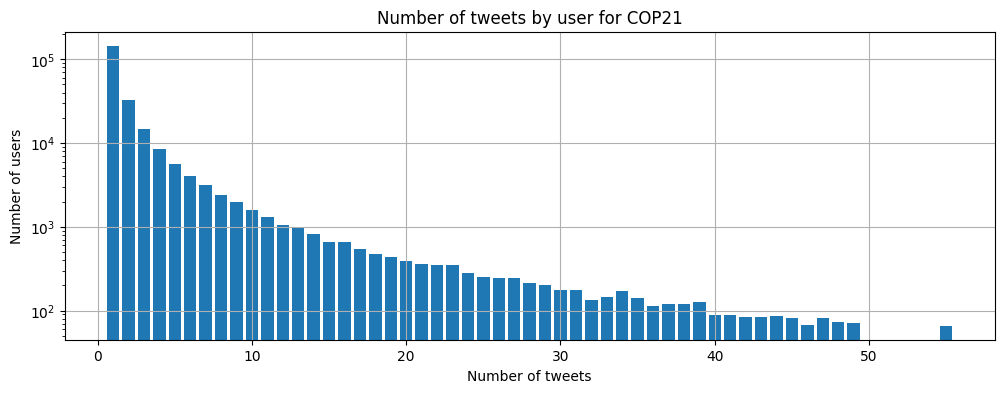
\includegraphics[width=0.75\linewidth ]{Chapter3/figures/tweets_by_users_cop21.png}

    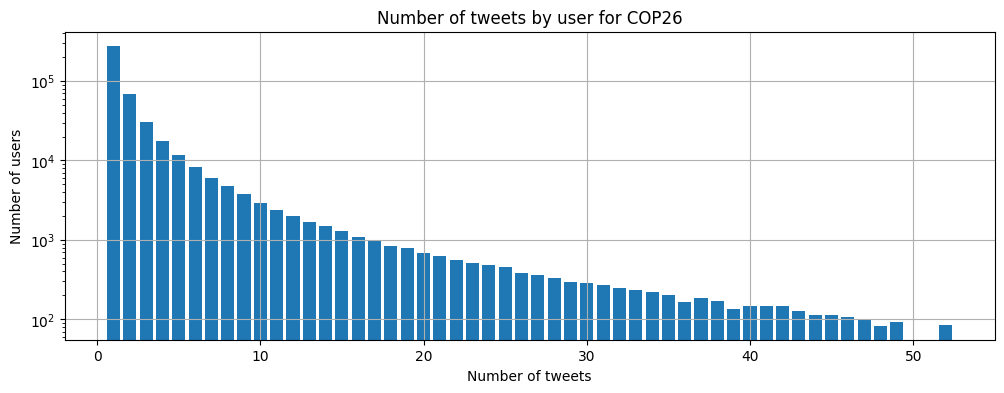
\includegraphics[width=0.75\linewidth ]{Chapter3/figures/tweets_by_users_cop26.png}
    \caption{Numebr of tweets by user for cop 21 and cop26}
    \label{fig:tweets_by_users}
\end{figure}






\begin{table}[h]
\centering
\setlength{\tabcolsep}{10pt} % Sets the horizontal padding
\renewcommand{\arraystretch}{1.5} % Sets the vertical padding
\begin{tabular}{
  |l|
  S[table-format=7.0,group-four-digits=true]|
  S[table-format=7.0,group-four-digits=true]|
  S[table-format=7.0,group-four-digits=true]|
  S[table-format=7.0,group-four-digits=true]|
}
\hline
 & {\textbf{n\_tweets}} & {\textbf{n\_retweets}} & {\textbf{n\_original}} & {\textbf{n\_original\_with\_retweets}} \\ \hline
\textbf{COP21} & 975040 & 562946 & 412094 & 138427 \\ \hline
\textbf{COP26} & 1558968 & 1191813 & 367155 & 130138 \\ \hline
\end{tabular}
\caption{Number of tweets}
\label{tab:n_tweets}
\end{table}




In fig \ref{fig:cop26_tweets_stats} we can see how the 1'558'968 are distributed, in fact 76\% of them are retweets generated by only 130k original tweets. It is also worth noting that almost 2/3 of the original tweets have 0 retweets.

\begin{figure}
    \centering
    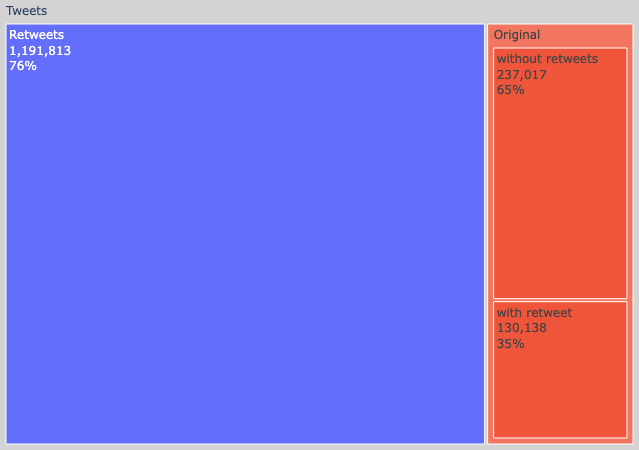
\includegraphics[width=0.9\linewidth]{Chapter3/figures/treemap_tweets-1.png}
    \caption{tweets of cop26}
    \label{fig:cop26_tweets_stats}
\end{figure}








% **************************** Define Graphics Path **************************
\ifpdf
    \graphicspath{{Chapter3/Figs/Raster/}{Chapter3/Figs/PDF/}{Chapter3/Figs/}}
\else
    \graphicspath{{Chapter3/Figs/Vector/}{Chapter3/Figs/}}
\fi


